%%%%%%%%%%%%%%%%%%%%%%%%%%%%%%%%%%%%%%%%%%%%%%%%%%%%%%%%%%%%%%%%%%%%%%%%%%%%%%%%%%%%%%%%%%%%%%%%%%%%%%%%%%%%%%%
\chapter{Energy preservation for SLM }
%%%%%%%%%%%%%%%%%%%%%%%%%%%%%%%%%%%%%%%%%%%%%%%%%%%%%%%%%%%%%%%%%%%%%%%%%%%%%%%%%%%%%%%%%%%%%%%%%%%%%%%%%%%%%%%
It can be proved that a restart of SLM does not alter the energy. This chapter is devoted to showing that this still hold with numerical approximations.

The residual energy of the symplectic Lanczos method is
\begin{equation}
\frac{1}{2} e_r^{\top} J A e_r + e_r^\top J r_{n+1} e_{2n}^\top z
\end{equation}
with $ e_r = u-u_n $ (analytical solution minus approximated solution) and $r_{n+1}$ is the residual vector given by the symplectic Lanczos method. 

\begin{figure}[H]
        \centering
        \begin{subfigure}[b]{0.45\textwidth}
                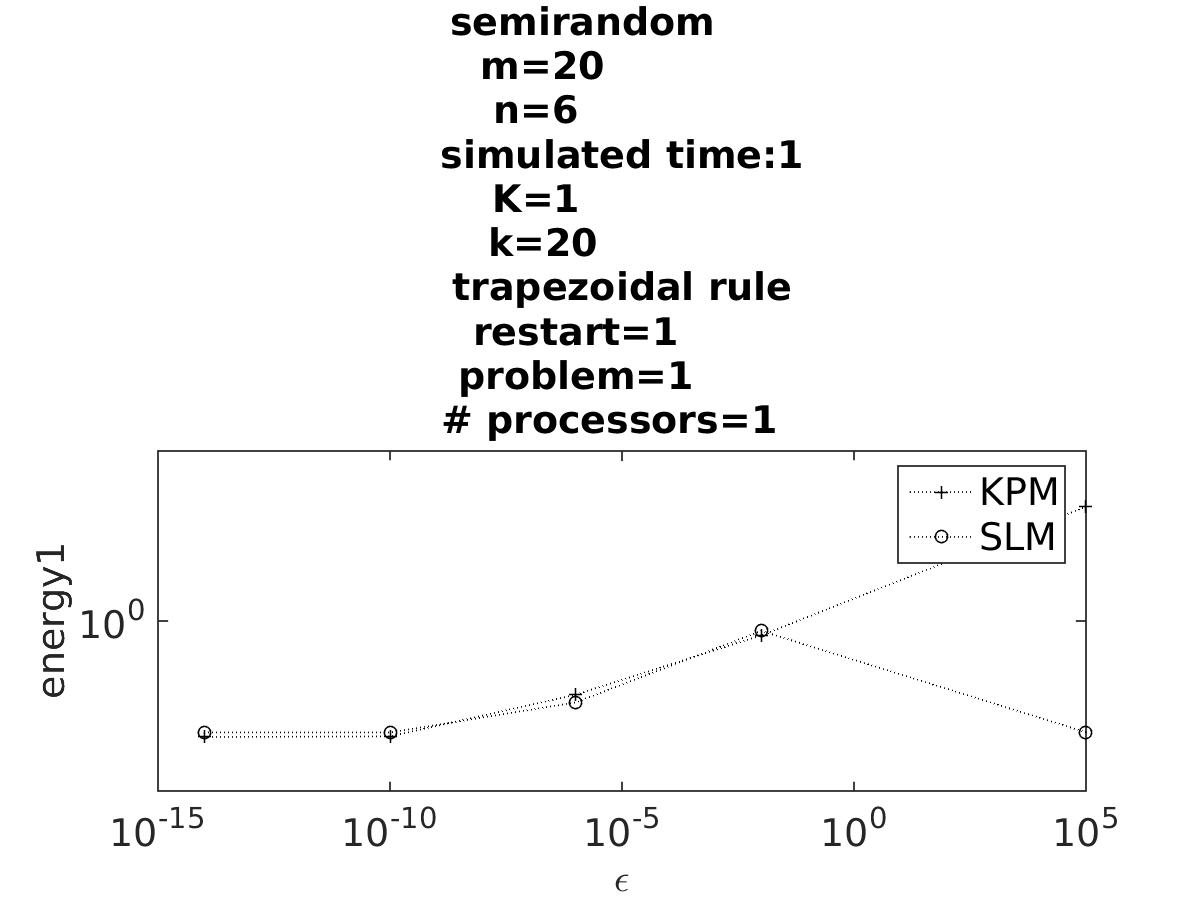
\includegraphics[width=\textwidth]{../MATLAB/fig/compareEnergy.jpg}
                \caption{ The difference in energy with and without restart. }
                \label{fig:compareEnergy}
        \end{subfigure}
        ~
        \begin{subfigure}[b]{0.45\textwidth}
                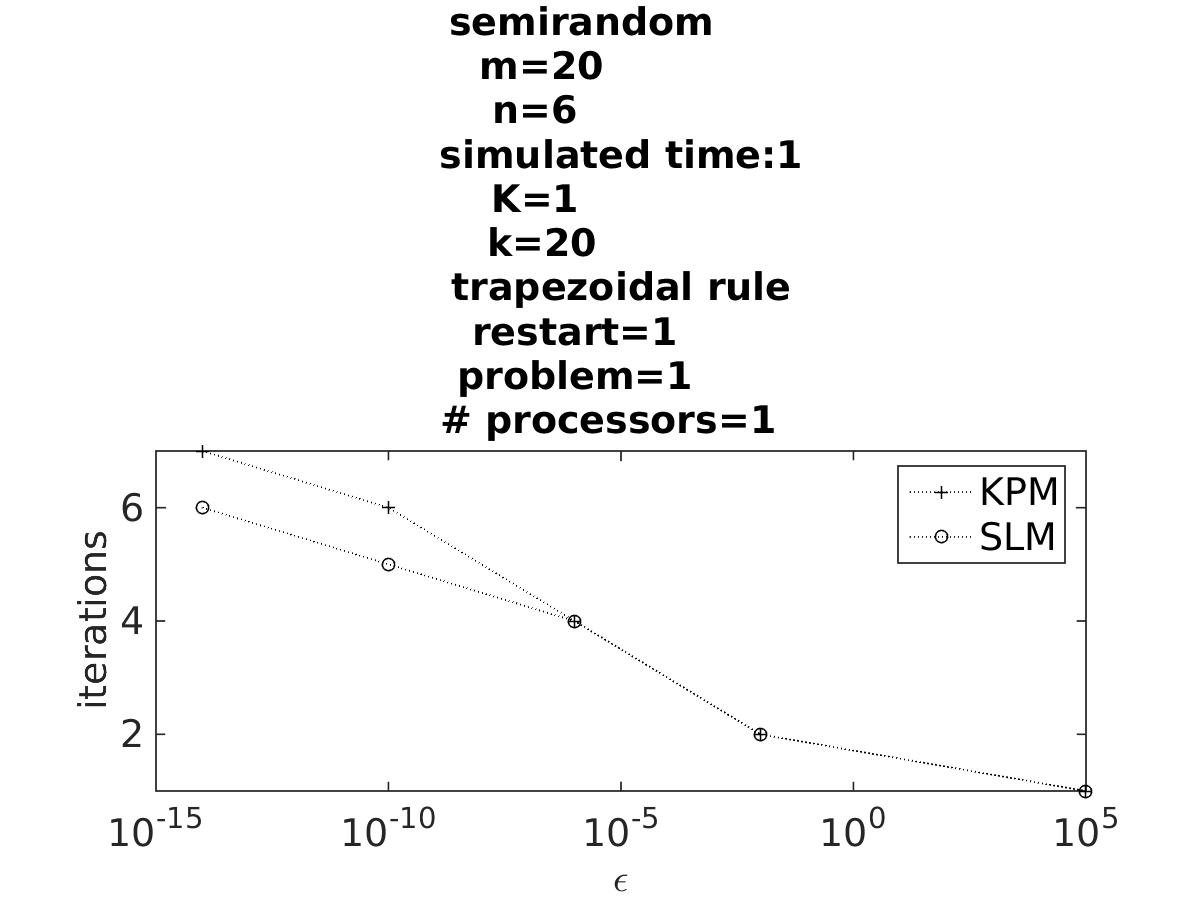
\includegraphics[width=\textwidth]{../MATLAB/fig/compareIter.jpg}
                \caption{ The number of iterations performed with and without restarting.  }
                \label{fig:compareIter}
        \end{subfigure}
        \caption{ The figure shows how the different methods change the energy with and without restarting.  }
        \label{fig:compare}
\end{figure}

The figures above implies that restarting the symplectic Lanczos method does indeed not change the energy. But for Arnoldi's method it changes quite a bit. 

\begin{figure}[H]
        \centering
        \begin{subfigure}[b]{0.45\textwidth}
                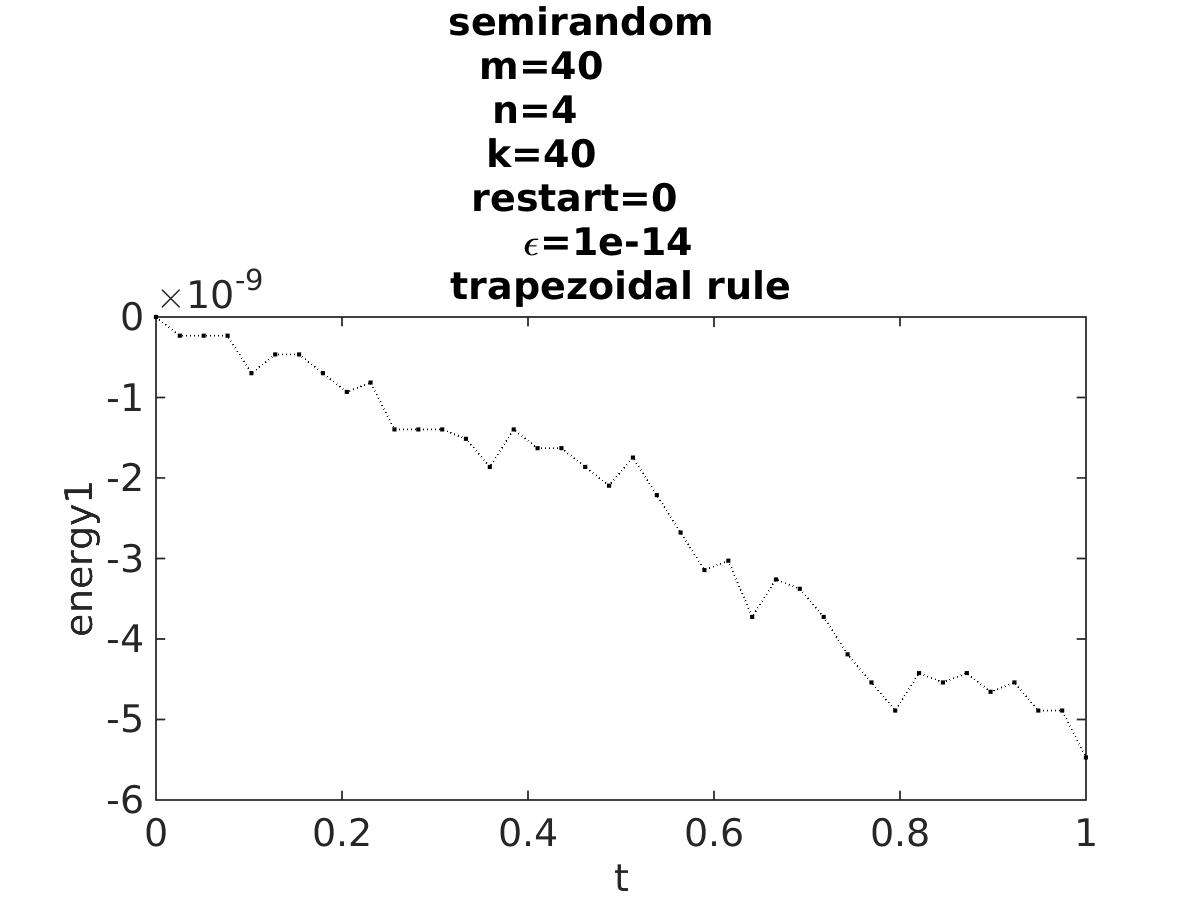
\includegraphics[width=\textwidth]{../MATLAB/fig/energytestrestart0.jpg}
                \caption{ Without restart. }
                \label{fig:energytestrestart0}
        \end{subfigure}
        ~
        \begin{subfigure}[b]{0.45\textwidth}
                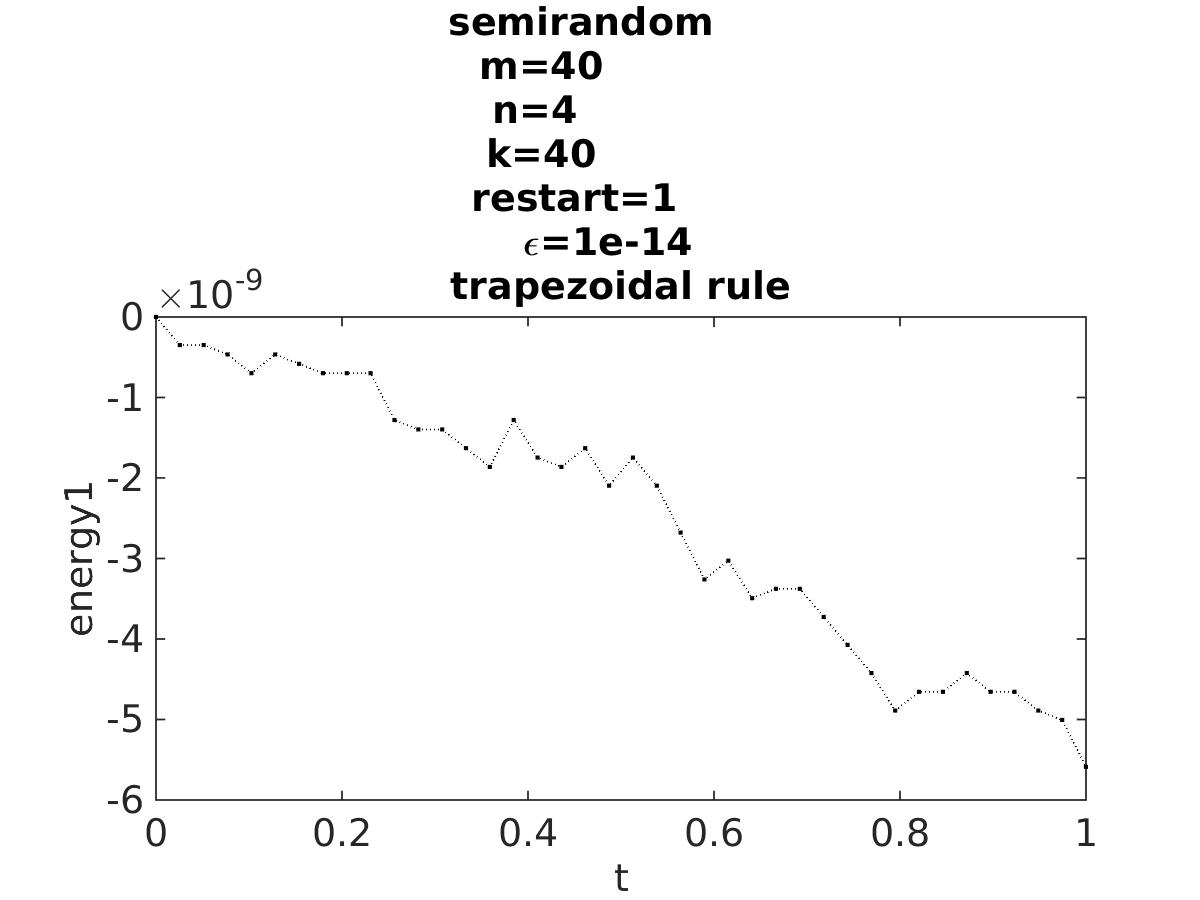
\includegraphics[width=\textwidth]{../MATLAB/fig/energytestrestart1.jpg}
                \caption{ With restart, the number of iterations $= 47$ }
                \label{fig:energytestrestart1}
        \end{subfigure}
        \caption{ The figures shows the change in energy over time. Mer tekst  }
        \label{fig:energytestrestart}
\end{figure}
The figure above shows very little change in energy with SLM, with and without several restarts. \\

The figures below shows the same as figure \ref{fig:energytestrestart}, but with KPM instead of SLM. 

\begin{figure}[H]
        \centering
        \begin{subfigure}[b]{0.45\textwidth}
                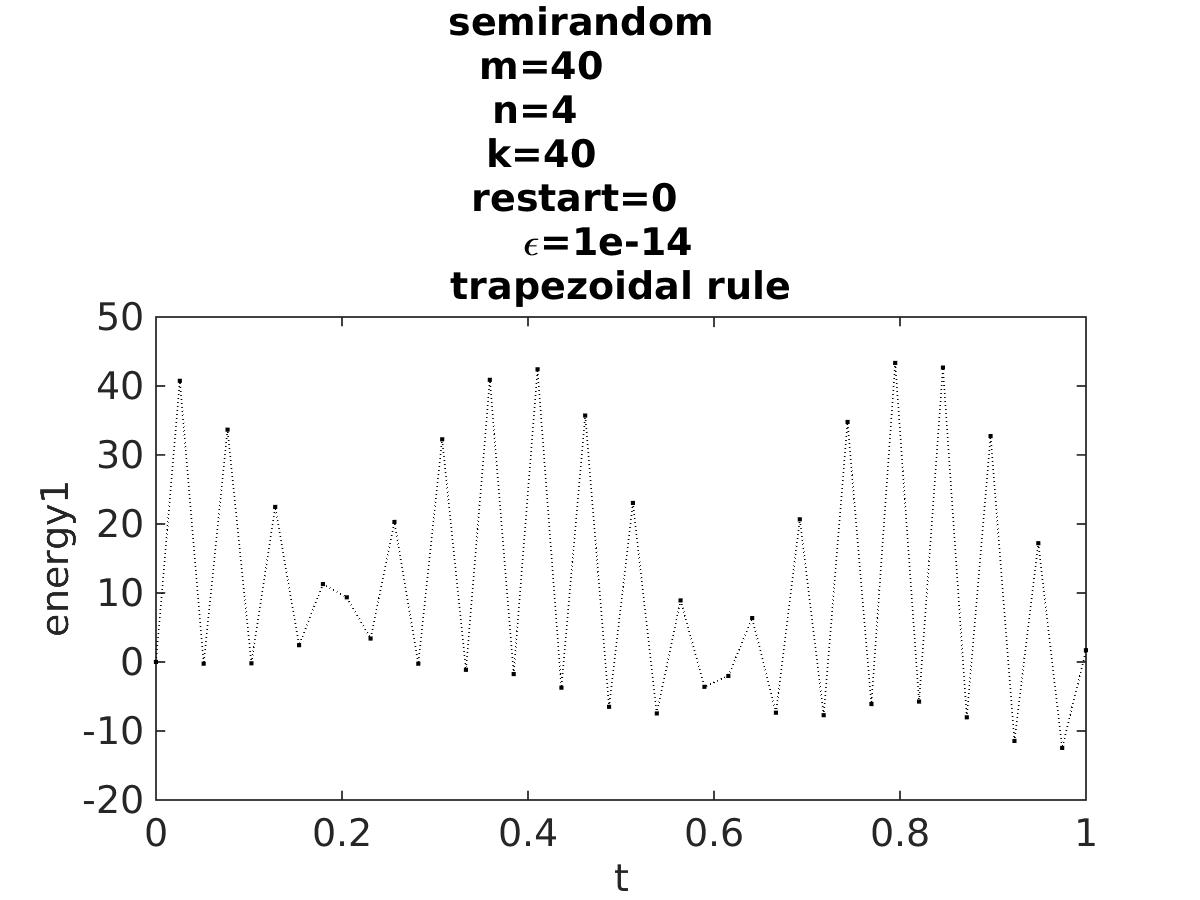
\includegraphics[width=\textwidth]{../MATLAB/fig/energyarnrestart0.jpg}
                \caption{  Without restart. }
                \label{fig:energyarnrestart0}
        \end{subfigure}%
        ~
        \begin{subfigure}[b]{0.45\textwidth}
                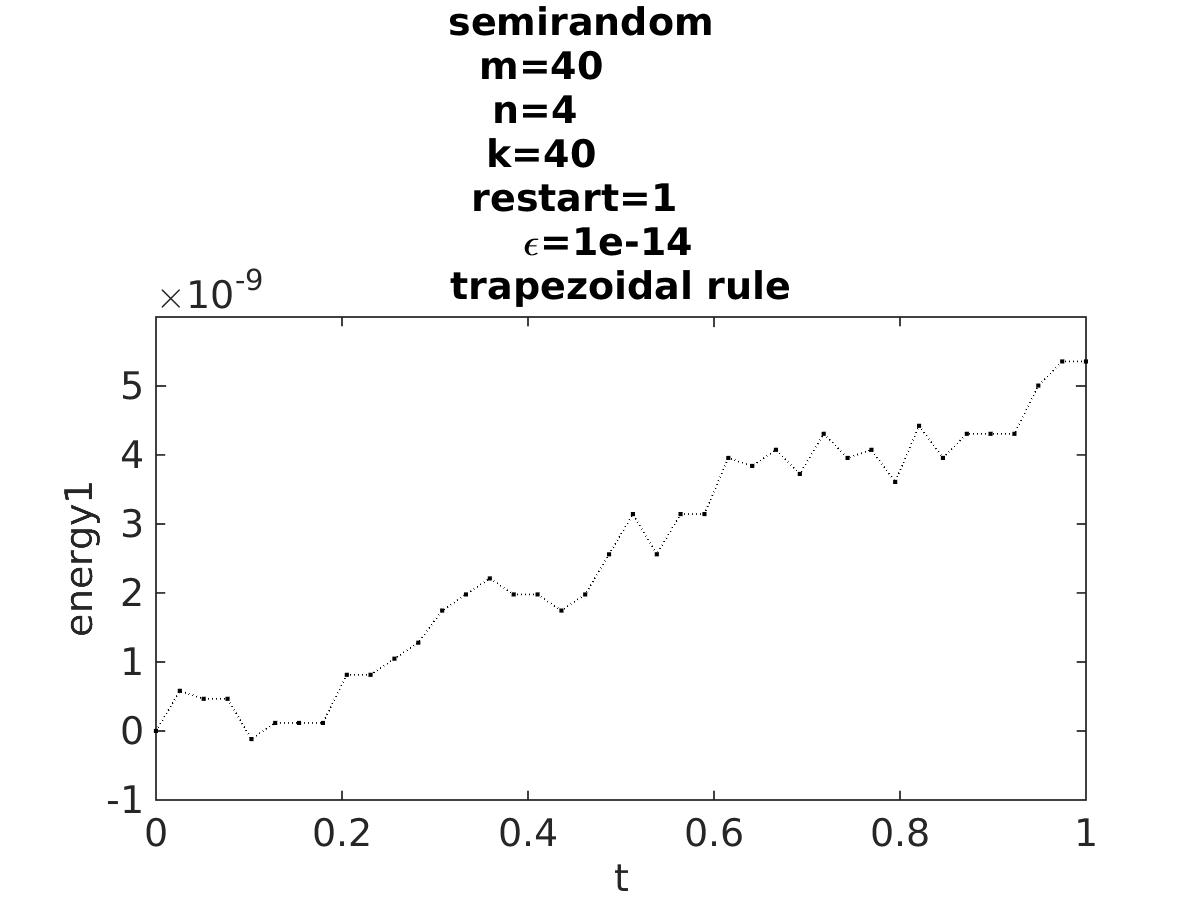
\includegraphics[width=\textwidth]{../MATLAB/fig/energyarnrestart1.jpg}
                \caption{ With restart, the number of iterations $ = 48$ }
                \label{fig:energyarnrestart1}
        \end{subfigure}
        \caption{ Figures showing the change in energy over time. Mer tekst  }
        \label{fig:energyarnrestart}
\end{figure}

When comparing figure \ref{fig:energytestrestart0} and \ref{fig:energytestrestart1} it becomes clear that SLM's does not alter the energy significantly when performing the restart. Figure \ref{fig:energyarnrestart0} and \ref{fig:energyarnrestart1} shows that this is not the case for KPM.\\

!!!!!!!!!!!!!!!!!!!!!!!ER dette overbevisende nok?!!!!!!!!!!!!!!!!!!!!!!!!!!!!!\\